% Options for packages loaded elsewhere
\PassOptionsToPackage{unicode}{hyperref}
\PassOptionsToPackage{hyphens}{url}
\PassOptionsToPackage{dvipsnames,svgnames,x11names}{xcolor}
%
\documentclass[
  abstract]{article}

\usepackage{amsmath,amssymb}
\usepackage{algorithm}
\usepackage{algpseudocode}
\usepackage{iftex}
\input{preamble.tex}
\hypersetup{
  pdftitle={Group polarization replications may be marred by high false discovery rates},
  colorlinks=true,
  linkcolor={blue},
  filecolor={Maroon},
  citecolor={Blue},
  urlcolor={Blue}}


\newcommand{\mupre}{\mu_\mathrm{pre}}
\newcommand{\mupost}{\mu_\mathrm{post}}

\newcommand{\sigmapre}{\sigma_\mathrm{pre}}
\newcommand{\sigmapost}{\sigma_\mathrm{post}}

\newcommand{\thetafit}{\theta^\mathrm{fit}}

\newcommand{\fdr}{\mathrm{FDR}}

\newcommand{\meanobs}{\bar{o}}
\newcommand{\meanobsemp}{\bar{\mathbf{o}}}
\newcommand{\meanobst}{\meanobs_t}
\newcommand{\meanobsjt}{\meanobs_{j,t}}

\newcommand{\meanobspre}{\meanobs_\mathrm{pre}}
\newcommand{\meanobspost}{\meanobs_\mathrm{post}}

\definecolor{myorange}{RGB}{240, 96, 0}
\newcommand{\mt}[1]{{\textcolor{myorange} {({\tiny MT:} #1)}}}

\usepackage{authblk}
\usepackage{etoolbox}
\usepackage{wrapfig}
\makeatletter
\title{Group polarization replications may be marred by high false discovery rates}
\makeatother
\author[1,*]{{Matthew A.~Turner}}
\affil[1]{\small Division of Social Sciences, Stanford Doerr School of Sustainability, Stanford University}

\author[2,3]{{Paul E.~Smaldino}}
\affil[2]{\small Cognitive and Information Sciences, University of California, Merced}
\affil[3]{\small Santa Fe Institute} 
% \vspace{2em}
\affil[*]{\small Correspondence: \href{mailto:maturner@stanford.edu}{maturner@stanford.edu}}

\date{}
\begin{document}
\maketitle
\begin{abstract}
\noindent 
\emph{Group polarization} is the name for a form of consensus where
members of a like-minded group become, on average, more extreme in their
opinions after discussing a topic. Group polarization is important because
it may increase social and political tensions if moderates become more
extreme. Decades of studies have replicated detections of group
polarization, typically using an ordinal scale to measure opinions.
However, these studies did not account for ordinal measurements, which can
result in spurious detections of opinion change.  Lacking original data we
can still calculate the probability that a published detection of group
polarization was spurious, i.e., to calculate the \emph{false detection
rate}.  Across 54 group polarization experimental conditions from ten
representative journal articles, we calculated false detection rates to be
between 0.52 and 0.88, with a median of 0.75, using a generative model of
group polarization experiments seeded with empirical data.  
We also use our model to develop experimental designs that
achieve an acceptable false discovery rate.  Much of group polarization
research may be unreliable. This analysis can help change that by enabling others to avoid this
hidden pitfall. More
broadly this work demonstrates one important way that replication success alone
does not imply epistemic reliability.
\end{abstract}

\renewcommand*\contentsname{Table of contents}
{
\hypersetup{linkcolor=gray}
\setcounter{tocdepth}{2}
\tableofcontents
}

\begin{center} \noindent\rule{4cm}{0.4pt} \end{center}
\clearpage

\begin{quote}
In our introductory social psychology course, 
we have for many years used the [group polarization experimental paradigm] as
a laboratory exercise. The exercise works beautifully, but one must be
careful to forewarn a class that [group polarization] does not occur with every 
group\ldots and that the effect is not large. 
\par\raggedleft(Brown, 1986, p.\cite[p. 205]{Brown1986})
\end{quote}

\begin{quote}
One of the most robust findings in social psychology is that of attitude polarization 
following discussion with like-minded others.
\par\raggedleft(Cooper et al, 2001, p. 267 \cite[p. 267]{Cooper2001})
\end{quote}

\begin{quote}
A medium effect size is conceived as one large enough to be visible to the naked eye.
\par\raggedleft(Cohen, 1988 \cite[p. 26]{CohenBook1988})
\end{quote}


\section{Introduction}\label{introduction}

If an extremist's opinion falls and it is measured with a Likert scale, will it
make a noise? The answer had better be yes if we want to properly measure opinion
change. Accurate measurements are critical
for developing rigorous and reliable methods to promote more centrist,
sustainable, and responsive governments and institutions
\autocite{Mason2018UncivilAgreementBook,Klein2020}. Unfortunately, social and
behavioral scientists have often used statistical methods 
that distort
opinion change when it's measured on an ordinal, Likert-style scale (e.g. -3
indicates ``Strongly disagree'', +3 indicates ``Strongly agree'', and 0 is
neutral)~\autocite{Liddell2018}. 
This includes research that Obama official and law professor Cass Sunstein
marshals to explain why ``people become extremists'' and why ``political and
cultural polarization'' is ``so pervasive in America''\footnote{From the
  Publisher's Summary. Sunstein does not make such general claims in the book,
  but does suggest that the research he reviews collectively provides
  a ``clue'' to explaining how
  ``facism...student radicalism...Islamic terrorism...[t]he Rwandan
genocide...[e]thnic Conflict.}
administration official and law professor Cass Sunstein writing a book called
*researchers construct

This work is motivated by a core conviction that better thinking leads to better
science. Theoretical clarity, careful measurement, and principled statistical modeling are not academic luxuries, but essential tools for empirical science. The group polarization literature has long suffered from ambiguities in theory, ordinal-to-continuous mismatches in measurement, and default inferential techniques that mask model non-identifiability. By reconstructing these issues from the ground up, this paper aims not only to assess the credibility of existing evidence, but to show that rigorous thinking — about what we measure, how we model, and what we can legitimately conclude — has direct, practical consequences for the claims we make about the social world.

\emph{Group polarization} is that essentially
measures how much being in an opinion echo-chamber the name given the social phenomenon of 
when a group becomes more extreme in mean opinion over
time, assuming the mean opinion is biased to one extreme to begin with.
\mt{now hit them with the real shit to intro the problem, our analysis, and
how this can be used constructively going forward.}

\mt{Seems like a good second paragraph structurally. We should give more
details about the scope of the study, group polarization and common
elements of experimental designs.} 
Group polarization experiments tend to employ a common set of design
elements incorporated in our computational model analysis. Group
polarization experiments mostly use ordinal (see exceptions
\cite{Blascovich1974,Blascovich1975,Blascovich1976,Keating2016}). The opinions (e.g., ``Do you approve,
disapprove, or neither approve nor disapprove of the current
administration's policies?''). Extremity only increases, though, assuming
that the mean opinion of the group is initially biased towards one extreme
or the other \autocite{Brown1986,Brown2020}. Group polarization is important
to understand rigorously, therefore, since if groups become increasingly
extreme over time, while group opinions are consolidated, this would
exacerbate political polarization between political opposition groups, which
is already undermines the ability of partisans in democratic governments to
work together. Dozens of studies and meta-analyses over decades have
apparently established the empirical reality of group polarization
\autocite{Moscovici1969,Myers1970,Isenberg1986,Sunstein2009,Sunstein2019}
\autocite[Ch. 5]{Brown2000}. We believe group polarization should occur in
certain contexts since more extreme group members are likely also to be more
stubborn \autocite{Guazzini2015,Lewandowsky2019}, which should pull
consensus to extremes \autocite{Turner2020}. However, many or most of the
evidence for group polarization relies on experimental designs that use
ordinal measurements that are then analyzed as if they were continuous.
Unfortunately, this procedure is unfortunately known to induce false
positives if it is not properly accounted for \autocite{Liddell2018}.


The null-consistency procedure functions as a test of model indistinguishability: it demonstrates that a reported group polarization effect could plausibly arise from a stable-latent process combined with changing opinion precision. This logic echoes foundational concerns in causal inference, where two competing models—one causal, one not—can imply the same observed data distribution and are therefore empirically indistinguishable without further assumptions \cite{pearl2000causality,spirtes2000causation}. In such cases, inference from observation to mechanism is invalid. Similarly, in psychometrics, it is well known that different configurations of latent traits and response thresholds can yield identical observed ordinal patterns, making the true structure unidentifiable without additional constraints \cite{borsboom2005measuring}. The present approach does not attempt to estimate the probability of false detection, but rather shows that under ordinal measurement, a null model can reproduce the observed pattern—rendering the result non-diagnostic of a true latent shift. This establishes a stringent standard: an effect must not only be detected, but shown to be incompatible with plausible null-generating mechanisms.



Experimental designs in group polarization studies share a certain
experimental boilerplate (Figure 1 --- NEED TO INCLUDE) with the goal of
testing the group polarization hypothesis that a group of like-minded
people will develop more extreme opinions on some salient topic over the
course of discussing some topic (Figure~\ref{fig:ModelSketch}). 
Group polarization experiments are thus
initialized by forming like-minded groups of people and surveying their
initial opinions on some topic. In some cases these initial opinions are
used for assigning participants to like-minded groups, but other methods
have been used, such as geographic location for producing, on average,
like-minded groups \autocite{Schkade2010}. Participants then discuss the
topic in their groups. After discussion, participant opinions are again
measured. Several studies we analyze here determined group polarization
occurred (i.e., defined a positive detection) only as a non-zero
difference in mean opinion, with no other statistical testing. Some
others performed null-hypothesis \(t\)-tests to test whether there was
enough evidence to reject the null-hypothesis that \emph{simple
consensus} occurredand not group polarization. In our meta-analysis
simulations, we measure simulated group polarization effect size in
terms of Cohen's \(d\), which is an abstraction beyond these two
practices from the group polarization literature that can also be used
to compare model fits between metric models that treat group
polarization measurements as continuous although they are ordinal, and
more appropriate statistical models that account for data ordinality.

% \begin{figure}
%   \caption{\textbf{Opinions are implicitly behavioral choices that are most consistent with some
%   complex aggregation of brain states and dynamics, and so are theoretically
%   continuous (A). Common components of a group polarization experiment.}
%   Participants first give their opinion in response to some prompt (B). Afterwards,
%   participants deliberate the topic (C). Participants then give their opinion again
%   (D). }
%   \centering
%     \includegraphics[width=0.65\textwidth]{Figures/Model/ModelSketchesA.pdf}
%     \includegraphics[width=0.7\textwidth]{Figures/Model/ModelSketchesB-D.pdf}
%   \label{fig:ModelSketch}
% \end{figure}


In this paper, we perform a meta-analysis of sixty detections of group
polarization from ten published research articles and show that
fifty-five of the sixty cannot be reliably identified as group
polarization. We show that these 55 are plausibly false detections
because they are equally well-explained by a \emph{simple consensus}
model, where the mean group opinion is unchanged by group discussion but
opinion variance decreases. Theoretically, consensus occurs when
sufficiently like-minded individuals influence, which decreases group
opinion variance \autocite{DeGroot1974,Turner2018}. Group polarization,
then, is consensus plus an overall increase in group opinion extremity,
i.e., an increase in mean group opinion after discussion. We use a novel
approach, described herein, that enabled us to identify continuous pre-
and post-discussion simple consensus opinion distributions that result
in data that appear to be group-polarized when opinions are drawn from
these distributions and measured with an ordinal scale. This approach
could be adapted for similar social psychological studies that used
ordinal measures to determine whether change occurred in distributions
of continuous psychological variables such as opinions and beliefs. For
social psychology and group polarization, this means that an accepted,
heretofore unquestioned, empirical fact must be re-evaluated.
Experimental designs in the field must be updated if we are to
rigorously understand whether and when group polarization occurs.

\subsection{Studies included in this
meta-analysis}\label{studies-included-in-this-meta-analysis}

We chose the ten studies guided by a desire to identify foundational
studies that contribute to the general consensus in social psychology
that group polarization reliably occurs across experimental
settings---one author of one of the ten journal articles is a law
professor who has written two trade books on group polarization to argue
that group polarization occurs in real-world settings in addition to the
laboratory, with political and other practical importance
\autocite{Sunstein2009,Sunstein2019}. We chose studies that either had a
significant influence on the study of group polarization and social
psychology, in terms of a high citation count or adaptation in
popularized trade books, or were designed to support one of four
prominent theoretical explanations of group polarization. The studies
must also have used an ordinal scale for measuring participant opinions
(all but a handful of exceptions use ordinal measurements to measure
group polarization; e.g.~blackjack bets
\autocite{Blascovich1973,Blascovich1976} and mock jury monetary damages
\autocite{Schkade2000}). We included at least one study that supported
or was motivated by one of four established theoretical explanations
(introduced below) of group polarization to show all have at least some
supporting evidence that must be discarded. We also included two studies
that lack a clear theoretical motivation. For the sake of orienting the
reader to the group polarization literature and as a useful organizing
feature for our analysis, we now introduce the theories that motivate
eight of the ten studies. To further orient the reader, we then provide
details of the experimental designs used to produce the 60 published
positive detections of group polarization across 10 research articles
that we scrutinize here. Group polarization experimental designs are
diverse and inconsistent with one another in many ways, which
complicates this or other potential meta-analyses and may imperil our
ability to rigorously understand how regular the group polarization
effect really is \autocite{Yarkoni2022,Almaatouq2022}.

The first theoretical explanation whose supporting findings we include
here is (1) social comparisons theory, which posits that an individual's
opinions are updated so they stand out in a group enough to be
``desirably distinctive'' (Myers, 1978, p.~562) but not too distinct to
be viewed as anti-conformist \autocite{Brown1974,Sanders1977,Myers1978}.
Second, \emph{persuasive arguments theory} posits that more extreme
individuals have a greater number of more convincing arguments for their
view, which draw more moderate group members to extreme opinions
\autocite{Burnstein1973,Burnstein1975,Burnstein1977}. Third, the
\emph{self-categorization theory} predicts that group polarization will
occur as more moderate individuals judge the mean group opinion to be
more extreme \autocite{Turner1989,Abrams1990,Krizan2007}. Fourth and
finally, the social decision schemes explanation posits that the
structure of \autocite{Davis1973,Zuber1992,Friedkin1999a}. We do not
evaluate or compare these theories here, though a simpler explanation
that extremists are more stubborn may be a more parsimonious explanation
consistent with these four alternatives
\autocite{Acemoglu2013,Guazzini2015,Turner2020}.

Each of the ten group polarization studies we analyze here varied
significantly in how groups were formed, how opinions were gathered, and
other details. There was significant variation across experimental
designs, participant population sizes, group sizes, and how like-minded
groups were formed in the first place. We review some of these details
below to provide the reader with some insight into the experimental
designs that produced what we show are plausibly false positive
detections of group polarization. We focus here on the questions that
were asked, how like-minded novel experimental groups were formed,
organizing our presentation by theoretical tradition.

\subsubsection{Details of experimental conditions included in this
meta-analysis}\label{details-of-experimental-conditions-included-in-this-meta-analysis}

\paragraph*{Atheoretical}

The first of ten studies we included in our meta-analysis was by
Moscovici and Zavalloni (1969) \autocite{Moscovici1969} who sought to
measure group polarization among groups of French high school students
who discussed domestic and foreign politics. Moscovici and Zavalloni
tested four conditions whether group polarization occurred for two
different questions and two different rating systems: participants were
asked their opinions on then-president Charles De Gaulle and their
opinion about foreign aid from the USA either in the ``Opinion'' setting
or the ``Judgement'' condition (see Table 4 on p.~132).

The second, relatively more recent article is Schkade, Sunstein, and
Hastie (2010) \autocite{Schkade2010} who used geographic location to
construct like-minded groups by running a group polarization experiment
in two cities in the state of Colorado in the United States: Colorado
Springs, whose residents historically voted for republican candidates,
and Boulder, whose residents historically voted for democratic
candidates. Discussion groups were formed in which they measured group
polarization when group members discussed global warming, affirmative
action, and same-sex civil unions.

\paragraph{Social comparisons}

In developing the social comparisons theory of group polarization
(described in Myers (1978) \autocite{Myers1978}), Myers and Bishop
(1970), writing in \emph{Science,} \autocite{Myers1970} sought to
measure group polarization among high school students in the United
States who discussed racial attitudes and Myers (1975)
\autocite{Myers1975} measured group polarization in groups of college
students discussing the quality of a faculty member in one condition,
and women's rights and issues in another condition.

\paragraph{Persuasive arguments}

\paragraph{Self-categorization}

\paragraph{Social decisions scheme}

The ten studies we included each tested several experimental conditions
meant to elicit group polarization in novel experimental groups, 60 in
total, which we briefly introduce here.\\

\subsection{Research overview}\label{research-overview}

To evaluate whether published detections of group polarization are
plausibly false we developed and combined formal and generative models
of group polarization to identify plausible simple consensus pre- and
post-discussion opinion distributions that seem like group polarization
when binned or measured on ordinal scales. Opinion distributions are
assumed to be normal. We define a \emph{simple consensus pair} of
\emph{latent opinion} distributions to be a pair of pre- and
post-discussion distributions where the mean opinion is constant, but
the pre-discussion variance is greater than the post-discussion
variance. A \emph{latent distribution} of opinions represents the
internal, unobservable distribution of opinions for a group or
collection of groups. The \emph{observed distribution} is the
distribution of reported ordinal opinion measurements. We then define a
\emph{plausibly false detection} of group polarization to be one where
the mean post-discussion observed distribution is greater in magnitude
(i.e., more extreme) than the post-discussion observed distribution's,
but both were measurements of a pair of latent simple consensus
distributions.

In the formal model, a simulated observed distribution is generated by
binning a latent distribution into a finite number of ordinal scale
bins, then integrating over the probability density in each bin. In the
generative model, an observed distribution is simulated by first drawing
participant opinions from a latent distribution, then counting the
number of opinions falling within each bin. The formal model is used to
identify which, if any, simple consensus pairs exist for a given
reported detection of group polarization through an optimization routine
that finds pre- and post-discussion variances that generate simulated
observations that appear to be group polarization (or reports a failure
to such variances). If the optimization routine finds a constant latent
mean that generates simulated observed group polarization, then we say
the published group polarization detection is plausibly false. If the
routine fails to find a constant latent mean that generates simulated
group polarization, then we cannot and do not claim the detection is
plausibly false. We use the generative model to evaluate how frequently
we would expect plausibly false detections when there are finite-size
groups, since the formal model implicitly applies infinite-size groups.
Therefore in our analyses, we also generate one thousand simulated group
polarization datasets for each of the 55 plausibly false detections
identified with the formal model and examine the distribution of group
polarization effect sizes in terms of Cohen's \(d\). In the first round
of simulations we set the number of observations to match those in the
ten published studies we analyzed. Many or most simulated effect sizes
are non-zero with these numbers of observations. To see if perhaps these
non-zero effects were due to low statistical power from too few
observations, we also tested a hypothetical study with ten times more
participants. Finally, we evaluate whether an appropriate statistical
model that accounts for the ordinal measurement of latent opinions can
reliably identify simulated simple consensus in latent opinions when
simulated observations appear as group polarization based on mean group
opinion alone.

% \begin{wrapfigure}{l}{0.5\textwidth}
\begin{figure}
  \caption{\textbf{Group polarization experimental model.} Latent opinions are 
    represented as numbers corresponding to the valence and extremism of one's opinion
(A). Before deliberating a topic of interest, all participants report their 
opinion (B). Participants then deliberate the topic with others (C). Following
deliberation participants report their opinion once more (D).}
  \centering
  \includegraphics[width=0.65\textwidth]{Figures/Model/ModelSketches.pdf}
  \label{fig:experiment_model}
% \end{wrapfigure}
\end{figure}

\section{Methods}\label{methods}

% We begin by developing a formal model of ordinal measurement of latent
% continuous opinions (model variables and parameters are given in
% Table~\ref{tab:modelVariables}).

Metascience frames our analysis since metascientific theory provides a framework for
our goal of calculating the false discovery rate across experimental conditions,
journal articles, and the ten-paper corpus. The false discovery rate is then
the Type I error rate relative to the rate of positive discoveries, true or false.
We calculate via simulation and data fitting
the Type I error rate for the experimental designs used in experimental conditions
that, under a preliminary large-$N$ model analysis, generated group
polarization upon ordinal measurement of simple consensus latent opinion 
distributions. These can then be aggregated to estimate the false discovery rate
for each journal article and for the ten-article corpus, which is representative of the
false discovery rate for group polarization studies. 

\subsection{Metascience of the false detection rate in group polarization}

The false detection rate is the scaled probability that a detection, $D$, of
an effect, $E$, is in fact a false detection and there is \emph{not} an effect,
denoted $\neg E$. The probability that a detection $D$ has occurred when there
was no effect, i.e. when $\neg E$, is denoted $\alpha = \Pr(D | \neg E)$.
This is known as the Type I or family-wise error rate. To calculate the 
false detection rate ($\fdr$), one must compare $\alpha$ to the statistical power,
the probability of a detection when there is an effect, denoted $W = \Pr(D | E)$.
Both these values must be scaled by the rate at which effects occur, denoted $b$.
Using the notation outlined above, the false detection rate is
\begin{equation}
  \fdr = \frac{(1 - b)\alpha}{(1 - b)\alpha + bW}.
  \label{eq:fdr}
\end{equation}


In group polarization, $E$ represents the group polarization \emph{effect}, and
$\neg E$ represents its absence. Simple consensus is one way for group polarization
to be absent, i.e., simple consensus is one form of $\neg E$. The presence of
an effect $E$ is independent of whether an effect was \emph{detected}, 
represented by $D$ if it was detected and $\neg D$ if not. 

The group polarization studies are journal articles that present
the results of multiple experiments to support some hypothesis. To organize
the presentation of false detection rates across the ten studies in our
analysis, we first will organize false detection rates by experiment, where
we created `ExperimentID` tags for each of the sixty experiments across ten
studies. We also created `StudyID` tags for each of the ten journal articles
with the key `{Author}{Year}`, e.g., \texttt{Schkade2010} for Schkade, et al.,
(2010) \cite{Schkade2010}. 

We calculate $\alpha = \Pr(D | \neg E)$ through simulation for experimental
conditions, 
and use optimistic values of
$b=0.1$~\cite{Ioannidis2005,McElreath2015} and $W=0.8$~\cite{Smaldino2016NatSel}
in the main text and in the compare with more pessimistic, yet realistic, estimates
of these values, as well as even more optimistic estimates. 

\subsection{How study design can induce false detections of group polarization}
\label{subsec:false-detections}


An opinion is never measured directly, only a behavior that indicates an opinion
in a behavioral experiment or survey.  For example, the location of a mark
that a participant makes is measured, not the complex neural activity that
underlies forming opinions (Figure~\ref{fig:experiment_model}A) \mt{Some of this
needs to be Intro'd}.
Theoretically, an internal opinion in the form of neural activity is a
\textit{latent opinion}, from the Latin \emph{latentem} meaning ``lie
hidden''.  Participants report \text{observed opinions}, typically as one of
a finite number of ranked, successive integer values that form the
\emph{selection set}. The minimum possible value in the selection set might
mean ``strongly disagree'' and the maximum value represents ``strongly
agree''.

% \begin{wrapfigure}{r}{0.5\textwidth}
\begin{figure}
  \caption{\textbf{Opinion measurement model and spurious group polarization.} 
  Latent model participant opinions are drawn from a normal distribution with the
  listed parameters (A,C). The pre-deliberation latent distribution has high
  variance, but appears polarized when measured via integration (A).  The latent
  distribution's variance is expected to decrease during deliberation (B) via
  consensus, but in this example the latent mean is static, 
$\mupre = \mupost$. However, when the post-deliberation distribution is measured,
the simulated observed mean increases, i.e., spurious
group polarization occurs (C).}
  \centering
  \includegraphics[width=0.65\textwidth]{Figures/Model/latent-ordinal-distros.pdf}
  \label{fig:distros}
\end{figure}
% \end{wrapfigure}

Group polarization experiments share a common experimental design where,
first, participant opinions are gathered on a topic of interest. Next, groups
are formed that have some initial opinion extremism. Participants deliberate
or discuss the topic for some set time. After the set time, participants
again give their opinion. Group polarization is said to occur if the
mean group opinion became more extreme, i.e., if the magnitude of the mean
group opinion is greater \emph{post-deliberation} compared to
\emph{pre-deliberation}. For example,
\cite{Moscovici1969} asked Parisian high school students to indicate their
degree of agreement with the statement, ``American economic aid is always
used for political pressure'' (Figure~\ref{fig:experiment_model}A). There
were seven options in the selection set, -3 indicating ``strongly disagree'',
+3 indicating ``strongly agree'', and 0 was neutral. Moscovici and Zavalloni
report that the mean pre-deliberation opinion was -0.61 and the mean
post-deliberation opinion was -1.09 (Moscovici and Zavalloni, 1969; Table 4,
p. 132). This is a -0.48 shift to more extreme disagreement with the 
statement, reported by Moscovici and Zavalloni as statistically significant
in Table 5 on p. 132.

We formalize this experimental design in the $N\to\infty$ case where the
distribution of ordinal measurements is created by integrating continuous latent
opinion distributions.  Latent opinions in the model are normally distributed with
mean $\mu_t$ and variance $\sigma_t$ for time $t$. We are concerned with only two
times, \emph{pre-} and \emph{post-} deliberation ($t=0$ and $t=T$, respectively).
For short we can write $\mu_\mathrm{pre}$ and $\sigma_\mathrm{pre}$ for
pre-deliberation mean and variance (and similar for \emph{post}-deliberation).  
The latent opinion of participant $i$ at time $t$ is drawn from a normal 
distribution in the model, 
\begin{equation} 
  o_{i,t} \sim p(o; \mu_t, \sigma_t) = \mathcal{N}(\mu_t, \sigma_t).
  \label{eq:opinionDistribution} 
\end{equation} 
\noindent 
Latent opinions are assumed to be normally distributed since they are unbounded 
aggregations of neurobiological activity. 

The measurement process with $N\to\infty$ participants is simulated by 
integrating the latent opinion distribution between ordinal bin thresholds, 
of which there are $B+1$, where $B$ is the number of opinion bins, with sequential
integer values $b$. In the Moscovici and Zavalloni (1969) example, $b \in
\{-3,-2,\ldots,2,3\}$ and $B = 7$.
Bin $b$ is defined by its lower and upper continuous-valued thresholds, 
$\theta_{b-1}$ and
$\theta_{b}$, respectively. Thresholds are given by the following equations
(and visualized as dotted lines in Figure~\ref{fig:distros}).
\begin{equation}
\theta_b = \begin{cases}
  -\infty         & \text{ if } b=0 \\
  \infty          & \text{ if } b=B \\
  b + \frac{1}{2} & \text{ otherwise.}
\end{cases}
\end{equation}
\noindent
With thresholds defined, the frequency of ordinal measurment $b$ at time $t$ 
is (Figure~\ref{fig:distros})
\begin{equation}
  p(b;~\mu_t, \sigma_t, B) = \int_{\theta_{b-1}}^{\theta_b} p(o; \mu_t, \sigma_t)
  do.
  \label{eq:ordinal-frequency}
\end{equation}

We can now define spurious group polarization and give examples of when it occurs.
First, the observed group polarization opinion shift is
\begin{equation}
  s = \meanobs_\mathrm{post} - \meanobs_\mathrm{pre}~,
  \label{eq:group-polarization}
\end{equation}
\noindent
where the expected value of observed opinions at time $t$ is
\begin{equation}
  \meanobst = \frac{1}{B} \sum_{b=1}^B b \cdot p(b; \mu_t, \sigma_t, B).
  \label{eq:meanobs}
\end{equation}
\noindent
\emph{Spurious} group polarization is when mean observed opinions seem to increase in 
extremity when the latent mean held constant. We simulate spurious
group polarization by setting $\mupre = \mupost = \mu$ and setting the variances
to values known to induce spurious group polarization. 
We explain how to find a constant latent mean, $\mu$, and pre- and post-deliberation
variances, $\sigmapre$ and $\sigmapost$, respectively, that generate spurious 
detections of group polarization in the next section. 
% We describe how we find $\mu$,
% $\sigmapre$ and $\sigmapost$ next in Section~\ref{sec:finding-variances}.


\subsection{Web app controls algorithm to find parameters inducing spurious group polarization} 

To calculate the false discovery rate for each experimental condition, we first must
identify a constant latent mean, $\mu$, and latent variances $\sigmapre$ and
$\sigmapost$ that generate observation distributions\mt{define earlier?} with
reported mean pre- and post-deliberation opinions and resulting shift $s$ (calculated
using Equation~\ref{eq:group-polarization}). Define the collection of these
parameters $\beta = \{\mu, \sigmapre, \sigmapost\}$. We identify $\beta$ through a
hillclimbing optimization algorithm that finds $\beta$ that minimizes the difference
between reported pre- and post-deliberation mean opinions and simulated ones
calculated with Equation~\ref{eq:meanobs}. 

The algorithm to find $\beta$ holds $\mu$ constant while searching for $\sigmapre$
and $\sigmapost$ that generate observed $\meanobspre$ and $\meanobspost$, within a
tolerance of $\pm10^{-3}$ (Algorithm~\ref{alg:hillclimbing}). 
The algorithm requires a researcher to specify an initial
guess for $\beta$ and auxiliary parameter settings, which generally vary between
experimental conditions.  Furthermore, the algorithm does not always produce
reasonable distributions with a given $\beta$, and sometimes it does not produce
spurious group polarization.  Therefore, it is necessary to sanity check the latent
and ordinal opinion distributions for the $\beta$ found by the algorithm. If all is
well, the experimental condition can be marked as plausibly spurious.  To tame the
complexity involved in data entry and model fitting for each of these sixty
experimental conditions, we developed a web application to input data from control
the algorithm and inspect its results (Figure~\ref{fig:webapp}). Web application code is
available online in our GitHub
repository\footnote{\url{https://github.com/mt-digital/gp-statmod/blob/main/GroupPolarizationStatmod/app.R}}.

\begin{algorithm}
  \caption{Routine to find latent mean and variance that generate spurious group polarization.}
  \label{alg:hillclimbing}
  \begin{algorithmic}

    \Require $\mu$, $\sigma$, $\bar{\mathbf{o}}$ 
      \Comment{Set latent mean, guess variance that yields, input empirical mean.}

    \Require $\epsilon$, $\delta$, $i_\mathrm{max}$ 
      \Comment{Hillclimbing tolerance, step size, and maximum iterations.}

    \State $\Delta \gets \meanobs(\mu, \sigma) - \meanobsemp$ 
      \Comment{Initialize simulation error.}
    \While {$\Delta^2 > \epsilon$ and $i < i_\mathrm{max}$} \Comment{Search until desired
    accuracy or max iterations reached.}
      \State $\sigma' \sim \mathcal{N}(\sigma, \delta)$ \Comment{Draw new variance to test.}
      \State $\Delta' \gets \bar{o}(\mu, \sigma') - \bar{\mathbf{o}}$ 
        \Comment{Calculate error using new variance.}
      \If {$\Delta' - \Delta < 0$}
        \State $\sigma \gets \sigma'$
          \Comment{Update $\sigma$ if the error is less than before.}
      \EndIf
      \State $\Delta \gets \bar{o}(\mu, \sigma) - \bar{\mathbf{o}}$
        \Comment{Update simulation error if $\sigma$ is updated.}
    \EndWhile \\

    \Return $\sigma$
  \end{algorithmic}
\end{algorithm}


\begin{figure}
  \caption{\textbf{Shiny web application for user-guided hillclimbing to find
  parameters that generate spurious group polarization.} This web application enables users to
create new analyses of experimental conditions from published studies. Users 
provide initial guesses for the algorithm to use as starting points in 
finding variances that generate spurious group polarization. Users inspect 
model fits provided by the algorithm, adjusting parameters if necessary, and
mark an experimental condition as ``Plausibly spurious'' if a reasonable fit
is indeed found.\mt{Maybe add some A, B, C guides to the figure and include
in parentheses here to go with the text?}}
  \centering
    \includegraphics[width=0.75\textwidth]{Figures/Model/WebApp.png}
  \label{fig:webapp}
\end{figure}


Note that so far, we have only identified cases where spurious group polarization plausibly
occurs in the asymptotic case where $N\to\infty$ ($N$ being the number of participants).
Experimental conditions yielding plausibly spurious group polarization warrant 
some suspicion. If there exists set of latent simple consensus 
parameters $\beta$ that create binned (Equation~\ref{eq:ordinal-frequency})
opinion distributions that naively seem to be group polarized, then the means
of at least some samples from these distibutions with empirical numbers of 
participants would also appear to be shifted consistent with group
polarization. This process itself does not tell us the false detection rate.
We use the identified simple consensus parameters to define pre- and post-deliberation
latent opinion distributions in simulated trials of group polarization 
experiments.


\subsection{Estimating and limiting false detection rates}

To calculate the false detection rate we begin by simulating 
pre- and post-deliberation 
opinions by drawing $N_e$ samples from normal latent opinion
distributions that generated spurious group polarization, i.e., with
parameters labelled $\beta_e$ found in the hillclimbing step. Binning these
random values simulates observations. $N_e$ is the number
of participants in experimental condition $e$. Each trial $i$ of $N_e$
simulated pre- and post-deliberation observations is then inspected to see
if spurious group polarization occurred in the simulation. Spurious group
polarization is determined by first inferring the latent parameters of each
simulated experimental trial by fitting an ordered probit model~\cite{Liddell2018}. 
The inferred parameters are then used to calculate the effect size for that
trial, Cohen's $d$, defined as~\cite[p. 331]{Liddell2018}
\begin{equation}
  d = \frac{\mupost - \mupre}{\sqrt{\frac{1}{2}(\sigmapost^2 + \sigmapre^2)}}.
  \label{eq:cohens}
\end{equation}
\noindent
The family-wise error rate is, $\alpha_{e} = \Pr(D|\neg E)$, is the 
fraction of trials, 
with $d_{ei} > d^*$ for the $i^\text{th}$ trial for experimental
condition $e$, written
\begin{equation}
  \alpha_e = \frac{1}{N_T} \sum_i^{N_T} \Theta(d_{ei}; d^*),
  \label{eq:study_aggregate}
\end{equation}
\noindent
where
\[
  \Theta(d_{ei}; d^*) = 
    \begin{cases}
      1 & \text{ if } d_{ei} > d^* \\
      0 & \text{ otherwise.}
    \end{cases}
\]
and $N_T = 1000$ is the number of trials. For simplicity we assume that the sign of
$d_{ei}$ is positive, meaning a shift to greater extremisim. It is possible that
$d_{ei}$ could be negative, indicating a shift to lesser extremity. Indeed we
observe many simulations with a shift to lesser extremity. For now we do not
include these as indicating a ``significant'' effect, which we return to in the
Analysis below.

To calculate the family-wise error rate
for a study, $s$ which contains several experimental conditions, $e$,
\begin{equation}
  \alpha_s = \frac{1}{|s|} \sum_{e \in s} \alpha_e
\end{equation}
\noindent
The mean across all results identified as plausibly spurious is 
\begin{equation}
  \alpha_\mathrm{all} = \frac{1}{|E|} \sum_{e \in E} \alpha_e.
\end{equation}
We finally may calculate the false discovery rate by plugging this $\alpha$
into Equation~\ref{eq:fdr} and assuming empirically-motivated values for 
base rate, $b$, and statistical power, $W$, as well as more pessimistic and
optimistic settings for base rate and power.

We close our Analysis by inverting this procedure to find what significance value
$d^*$ is necessary to achieve a low family-wise error rate $\alpha_e = 0.05$ for
experimental condition, $e$. To do this we first calculate $\alpha_e(d^*)$ for a
sufficiently wide range of $d^*$. We then find the lowest $d^*$ for which
$\alpha_e(d^*) \leq 0.05$.


\section{Analysis}\label{analysis}

Our analysis estimates how the probability that a published detection of group
polarization is actually a false detection. We first identified latent opinion
parameters that yield spurious group polarization in an asymptotic $N\to\infty$
model. This gives us our first suggestion that experimental conditions may be
plausibly false. Briefly, we identified latent opinion distribution parameters
that generated spurious group polarization in 54 out of 57 experimental
conditions. In other words, 95\% of all group polarization detections are
plausibly spurious due to ceiling artifacts from the continuous latent
opinions-ordinal measurement experimental design. We then analyze the family-wise
error ($\alpha$) and false detection rate (FDR) 
for each experimental condition and aggregated 
up to the study level and across all studies and experimental conditions. 
We estimate the lower twentieth percentile of experimental conditions 
have \emph{at least} $\alpha \leq 0.16$, 
with median $\alpha \geq 0.27$ and upper eightieth percentile with $\alpha \geq
0.40$ (Table~\ref{tab:quantiles}\mt{A.  –but don't have A and B; TODO: separate
FWER and FDR tables, only use 0, 20, 50, 80, 100 for probs. Rename 0 -> min, 100 ->
max.}). For the fiftieth and eightieth percentiles this
corresponds to false discovery rates of 0.75 and 0.82, respectively. 
We emphasize that these estimates and others detailed below are lower bounds on
$\alpha$ and FDR since we are using what is likely an overgeneralized,
underspecified statistical model that does not account for all the potential
variance in experimental outcomes, which would increase error rates.
We close our Analysis by calculating which $d^*$ limits family-wise error rates to
$\alpha \leq 0.05$. This is greater than $d^* = 0.8$, classically taken to 
represent ``high'' significance, in all but six experimental conditions.

\subsection{Nearly all group polarization detections are plausibly spurious}

We used our formal distribution model of group polarization experiments
to identify plausible latent simple consensus distributions that generate spurious
group polarization in observed ordinal distributions 
in the asymptotic case of taking $N \to \infty$ ordinal measurements.
Across the ten studies we analyzed, we excluded 3 out of 60 experimental
conditions that did not claim to be positive findings of group polarization.
Of the remaining 57, we identified simple consensus $\beta$ that generate spurious
group polarization in 54 experimental conditions. In the other three, we did
identify $\beta$ that generate spurious group polarization, but the initial
simulated distributions were highly polarized. We rejected $\beta$ generated for
two spurious group polarization from Schkade, et al., (2010) because
the histogram plots of the observed opinion distributions are not
polarized~\cite[Figure 1, p. 234]{Schkade2010}. The other condition where we
found but rejected spurious group polarization $\beta$ was in a question 
about a ``bad teacher'' in Myers (1975)~\cite{Myers1975a}, where lower values
signify increasingly worse impressions of the teacher and higher values signify
increasingly good impressions. It is unlikely that a
``bad teacher'' would be rated as good in this case, so we excluded this 
from our analysis as well. This exclusion may be overly generous since Myers (1975)
did not provide details beyond mean values and opinion shifts, and the article was
published before open data practices.


\subsection{Half of experiments exceed a 70\% false discovery rate at ``medium'' significance}

We simulated trials from each experimental condition, $e$, by sampling and binning
pre- and post-deliberation latent opinions from distributions with parameters
identified with the $N\to\infty$ model as causing plausibly spurious group
polarization. For each $e$, we drew a number of samples equal to the number of
participants in the original experiments, $N_\mathrm{emp}$. To estimate family-wise
error and false detection rates, we fit an ordered probit model to the simulated
observations and obtained estimates of the group polarization effect size, $d$
(Equation~\ref{eq:cohens}). If the effect size was greater than a significance
value, $d > d^*$, then by definition there was a detection $D$ of group
polarization, even though there was no effect by design, written $\neg E$.  The
family-wise error rate is $\Pr(D|\neg E)$, calculated as the frequency with which $d
> d^*$ out of 1000 simulation trials. The false detection rate is the family-wise
error rate scaled using the base rate of effects and the statistical power
(Equation~\ref{eq:fdr}). We test three difference significance values, $d =
0.2,~0.5$ and $0.8$, corresponding to what Cohen prescribed to use for ``low'',
``medium'', and ``high'' significance. If not otherwise noted, we set the base
rate to be $b=0.1$ and the power $W = 0.8$ as metascience parameters to calculate 
the false discovery rate (Equation~\ref{eq:fdr}). Note that if the family-wise error
rate is low at $\alpha = 0.05$, the false discovery rate is $\fdr = 0.36$.

Different conditions yield different effect size distributions
(Figure~\ref{fig:effect_size_distros}), which 
determine the magnitude of error rates and difference between the error rates for low,
medium, and high significance values $d^*=0.2,0.5,0.8$ magnitude of error rates 
(Figure~\ref{fig:fwer_fdr_synthesis}B). 
Family-wise error rates varied from a minimum of one in ten for the
\texttt{Feminists-Experimental} condition from Myers (1975)~\cite{Myers1975a}
to a maximum of two in three for the \texttt{COSprings-CivilUnions} condition from
Schkade, Sunstein, and Hastie (2010)~\cite{Schkade2010} under medium
significance effect size $d^* = 0.5$ (Figure~\ref{fig:fwer_fdr_synthesis} and
Table~\ref{tab:quantiles}). The median family-wise error
rate is 0.28 for Krizan and Baron's (2007) experimental condition
\texttt{NoOutgroupScenario1}~\cite{Krizan2007}. This translated to a minimum
false detection rate of 0.52 for the Myers (1975) condition, a maximum false
detection rate of 0.88 for the Schkade, et al., (2010) condition, and a median false
detection rate of 0.75 for the Krizan and Baron (2007) condition. 

\begin{table}[ht]
  \caption{{\textbf{Quantiles for the two error-rate measures under different
  significance values.}}}
  \label{tab:quantiles}
  \centering
  % latex table generated in R 4.3.3 by xtable 1.8-4 package
% Tue Dec 31 16:29:18 2024
\begin{tabular}{lcccccc}
  \toprule
Measure & $d^*$ & Min & 20\%    & 50\%     & 80\%    & Max \\ 
  \midrule
   & 0.20 & 0.14 &  0.25  & 0.34   & 0.41  & 0.69 \\ 
  FWER, $\alpha$ & 0.50 & 0.07 &  0.16  & 0.23   & 0.30  & 0.60 \\ 
  & 0.80 & 0.03 &  0.10  & 0.15   & 0.21  & 0.46 \\ 
  \hline
  & 0.20 & 0.60 &  0.74  & 0.79   & 0.82  & 0.89 \\ 
  FDR  & 0.50 & 0.43 &  0.64  & 0.72   & 0.77  & 0.87 \\ 
  & 0.80 & 0.23 &  0.53  & 0.63   & 0.70  & 0.84 \\ 
   \bottomrule
\end{tabular}

\end{table}

In the conditions
with lower family-wise error rates, there were several conditions where using the low 
significance value $\alpha$ resulted in a much greater error rate than the medium or 
high significance values. In the ten conditions with the lowest $\alpha$ for 
$d^* = 0.5$, with $\alpha$ near 0.1, five of these conditions have $\alpha > 0.25$
when $d^* = 0.2$ corresponding to a small effect size. For low $\alpha$, the
difference in false detection rates for each $d^*$ value are more widely
distributed, following the distribution of $\alpha$, meaning that 
a modest increase in $d^*$ can have greater effects on the false discovery rate. In
the conditions above the 50th percentile, $\alpha$ approaches and exceeds one in
two, even when requiring ``high'' significance with $d^*=0.8$. With $d^* = 0.8$,
$\alpha$ approaches and exceeds one in four, with four near one in two. When 
requiring ``low'' signifance, 

Experimental designs within each study or article tend to share certain
characteristics, such as the number of bins in the ordinal measurement design
or the number of participants per condition. Therefore, the 
average false detection rate across experimental trials within a study
(Equation~\ref{eq:study_aggregate}) show that 

\begin{figure}

  \caption{\textbf{Family-wise error rates and false discovery rates across studies and experiments for
    low, medium, and high Cohen's $d$ significance.}}
  \label{fig:fwer_fdr_synthesis}

  \centering
  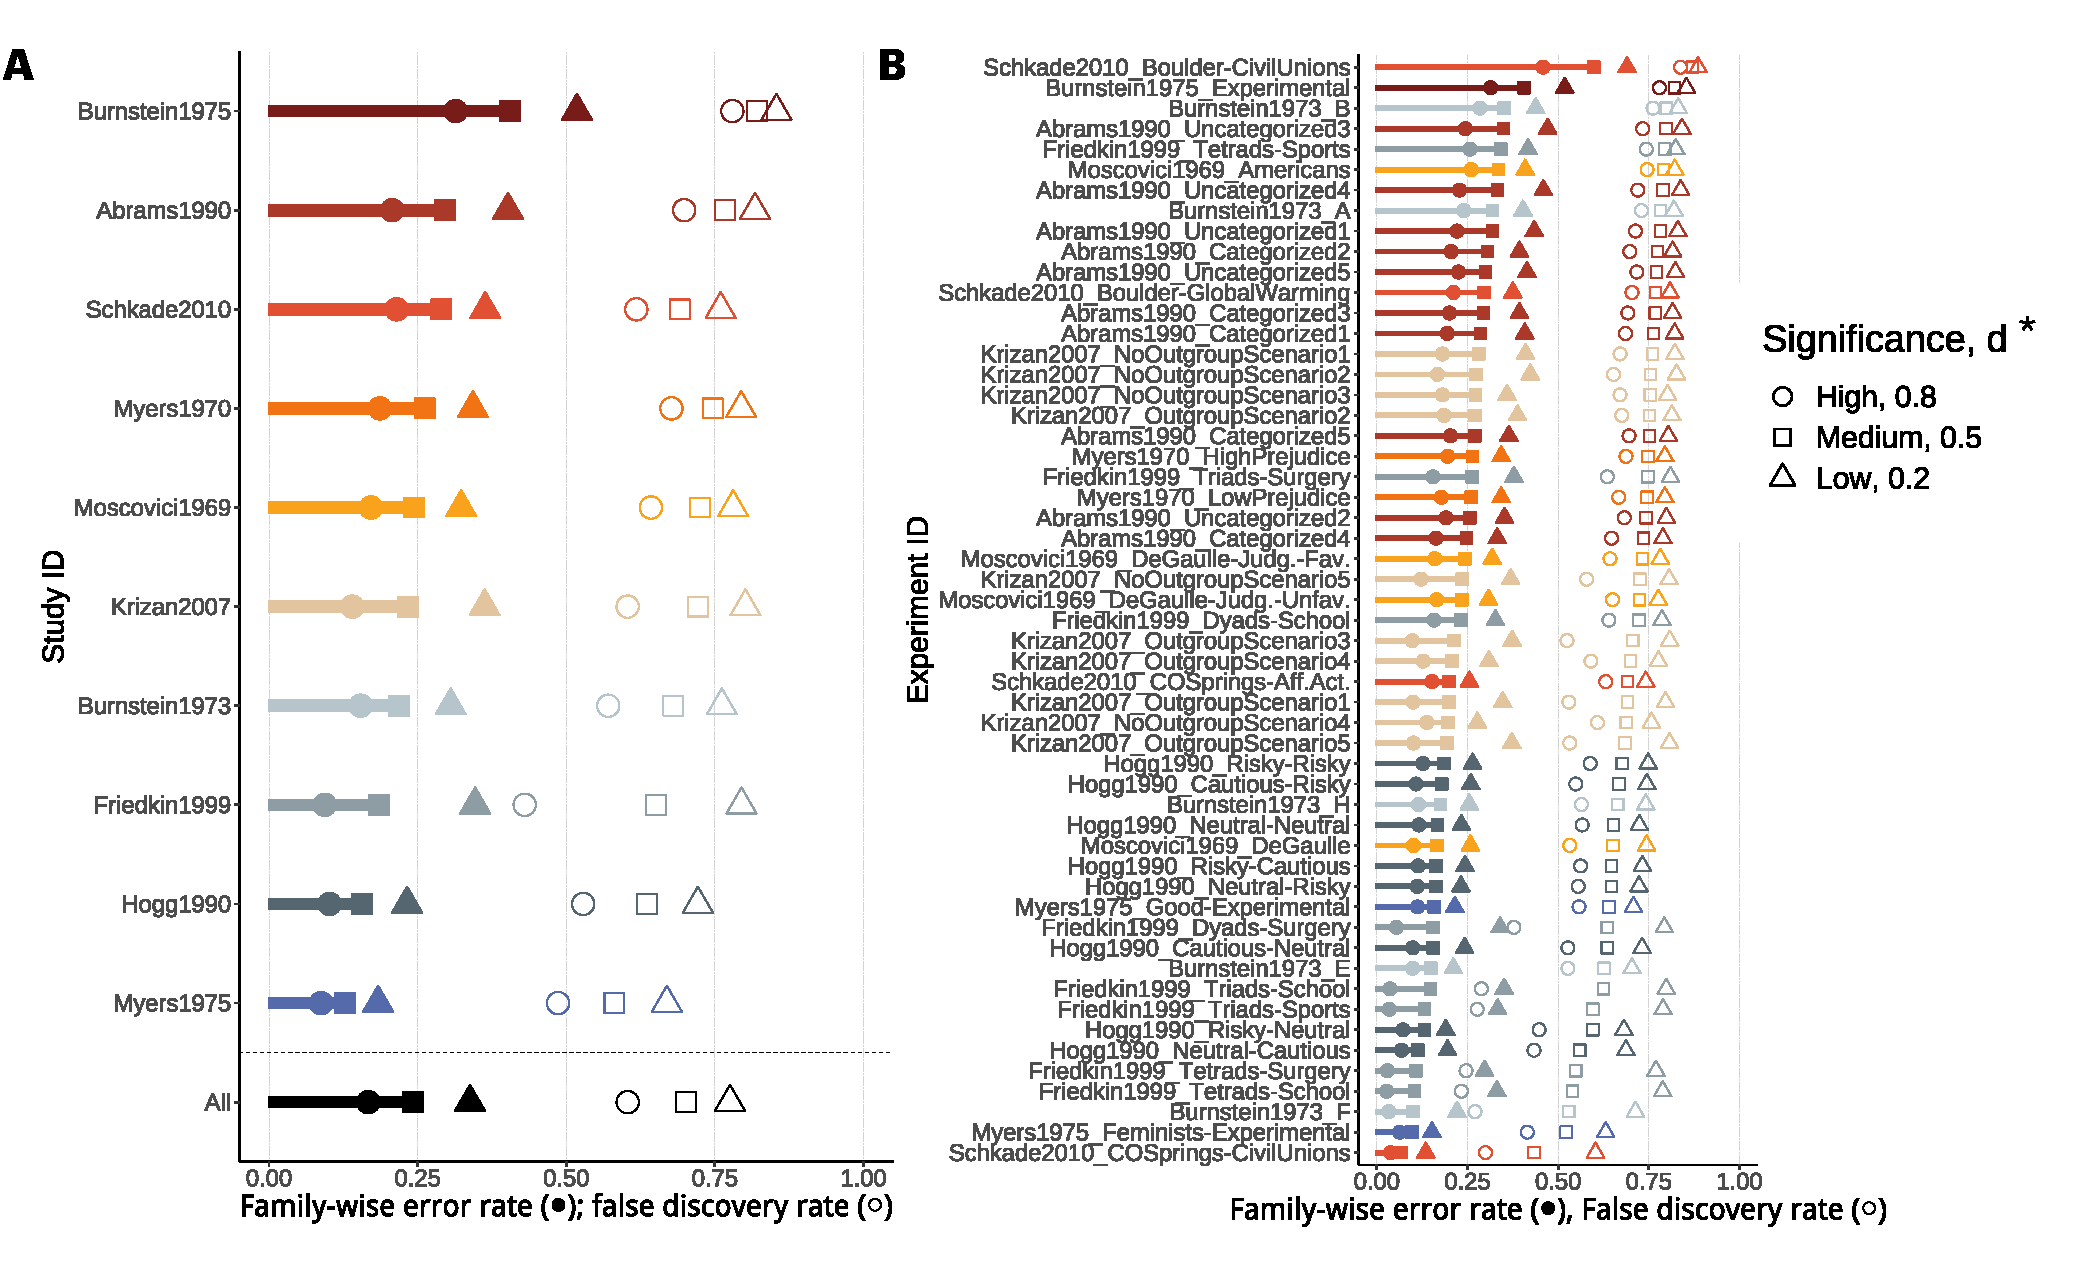
\includegraphics[width=1.1\textwidth]{Figures/Analysis/fwer_fdr_synthesis.pdf}
\end{figure} 

\begin{itemize}
  \item 
    Other $b$ and $W$ values in quantiles.
  \item
    Note that there were many ``significant'' results---in the wrong direction
    (Figure~\ref{fig:OrdinalBoxplot}).
\end{itemize}

\subsection{High significance values ($d^*$) often necessary for FWER of 0.05}

Our simulations can be used a different way, in this case to calculate what
significance value $d^*$ limits the family-wise error rate to the low value of
0.05. 
Solving the inverse problem of which $d^*$ achieves a low family-wise error rate,
which drives the false detection rate. Here we present our calculations to find
$d^*$ that achieve $\alpha(d^*) = 0.05$. 


\begin{figure}
  \caption{
    \textbf{Significance value, $d^*$, to limit family-wise error 
    rate of 0.05 for each identified study.} The Moscovici and Zavalloni (1969)
    ``Americans'' question would require the greatest $d^*$ to achieve $\alpha \leq
    0.05$, even though it does not have the highest error rates. This is because of
    larger outliers in simulated $d$ for this condition compared to others with
    greater error rates (Figure~\ref{fig:OrdinalBoxplot}).
  }
  \centering
    \includegraphics[width=0.75\textwidth]{Figures/Analysis/sigval_for_low_fwer.pdf}
  \label{fig:sigval_for_low_fwer}
\end{figure}



\section{Discussion}\label{discussion}

\mt{Restate results and importance and outline this section.}

\mt{One more brick to fall in the ongoing replication and generalizability crisis \autocite{Yarkoni2022}.}

Since there seems to be no selection pressure on false discovery rates, 
experiment design for studying group polarization was free to evolve randomly.
Various choices for the number of bins and other instrumental details may have
then become entrenched in different communities defined by 
common theoretical perspectives taken by researchers in those communities. 
Therefore, when 
Isenberg (1986)~\cite{Isenberg1986} reports that his meta-analysis found more
support for the XX theory than the YY theory in the form of greater effect sizes,
it may just be random cultural drift that the XX community instruments had higher
intrinsic false detection rates. In some cases it may be debatable whether to
control for the Type I error rate, or may depend on context~\cite{Rubin2021}. 
In this context, however, it is clear that we must apply such selection pressure 
to group polarization experiments or it may be nearly impossible to trust 
statistical analyses of these studies.

This leads to one of many follow-up research questions generated by this work.
First, are there general principles of experimental design that could reduce
the false detection rate for group polarization or similar experimental protocols?
Second, what is the best way to calculate false detection rate? 
Likely, even if we cannot identify parameters consistent with simple consensus
that generate spurious group polarization shifts in the large $N$ case, one
may still guess at some simple consensus parameters and caluclate the false
detection rate as we did. On the flip side, we likely found only one of infinitely
many simple consensus parameters that could result in a false detection. Does this
have an effect on the calculated false positive rate? More generally, our
work motivates similar analyses of sub-fields of social 
psychology and that do not account for Likert-based experimental designs in
their statistical analyses. We provided a template for this future work.

Our analysis brings some additional questions into focus. Most significantly, recall that even
the more appropriate ordered probit Bayesian model often failed to accurately detect negative
results with the number of participants used in the original papers. Many of the studies
analyzed here did not use any statistical test to establish significance; those that did used
some form of a $t$-test, and it is not clear if the $t$-test that was used 
accounted for a change in pre- and post-deliberation opinion variance, which we expect due to
consensus.

The ordered probit model we used still likely underestimates the variance in outcomes, which
could require even larger sample sizes. A more rigorous analysis
would include additional sources of variance that will likely further inflate the Type I
error rate, $\alpha$, and the false discovery rate~\cite{Yarkoni2022}. First and foremost,
there is variance within each experimental deliberation group; no group polarization study
accounts for this, instead treating participants in each experimental condition as if they were
one large group. Furthermore, survey data are known to be noisy~\cite{Zaller1992}. People
report opinions differently over time for no apparent reason (i.e., opinions are
\emph{unstable}).  Context matters: the order in which a survey question is asked, and which
question framing is chosen among logically equivalent alternatives, can both significantly
influence participant responses. The effect of accounting for these sources of variance must be
understood to estimate $\alpha$ (and power, $W$) for the design of the next generation of group
polarization experiments.

\mt{concluding paragraph: first sentences summarize the Discussion, then
in 1-2 sentences summarize the paper.}

\printbibliography[title=References]

\appendix

\renewcommand{\thefigure}{A\arabic{figure}}

\setcounter{figure}{0}

\clearpage

%%%%%%%%%% Supplement %%%%%%%%%%
\pagebreak
\begin{center}
  \textbf{\Large \textsf{Group polarization replications may be marred by high false discovery rates (Supplementary Material)}}
\end{center}

%%%%%%%%%% Prefix a "S" to all equations, figures, tables and reset the counter %%%%%%%%%%
\setcounter{equation}{1}
\setcounter{figure}{0}
\setcounter{section}{0}
\setcounter{table}{0}
\setcounter{page}{1}
\makeatletter
\renewcommand{\theequation}{S\arabic{equation}}
\renewcommand{\thefigure}{S\arabic{figure}}
\renewcommand{\thetable}{S\arabic{table}}
\renewcommand{\thesection}{S\arabic{section}}
\renewcommand{\thepage}{S\arabic{page}}

\section{Analysis}

\begin{figure}
  \caption{Boxplot of Cohen's $d$ for the ordered probit model over 1000
    simulation trias for each experimental condition (y-axis in A and B). Each
    trial represents a possible outcome of a group polarization experiment where
    the true opinion shift is zero. The mean across trials is closer to 0 than
    in the metric case, but many simulated zero-shift experiments still result in
    an observed shift. This illustrates the weak statistical power of these group
    polarization experiments.}
  \label{fig:OrdinalBoxplot}
  \centering
    \includegraphics[width=1.0\textwidth]{Figures/Analysis/ordinal_cohens.pdf}
\end{figure}


\end{document}
